\documentclass[border=5pt]{standalone}
\usepackage{tikz}
\usepackage{amsmath}
\begin{document}
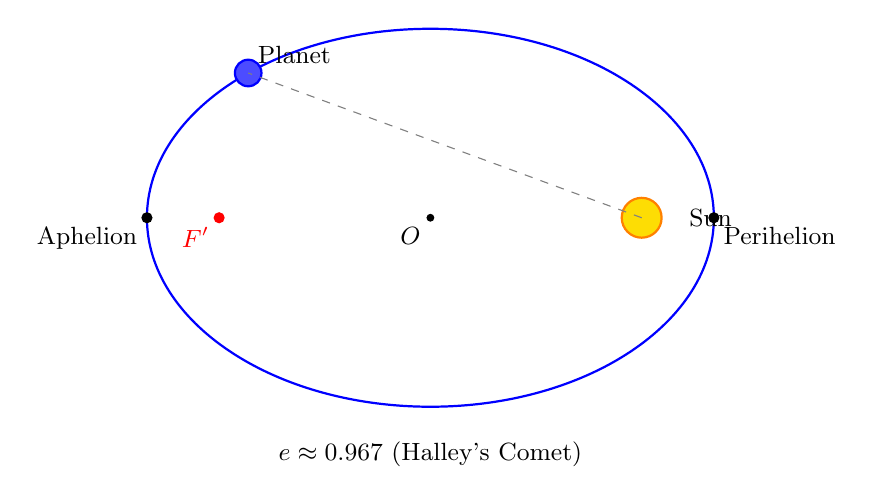
\begin{tikzpicture}[scale=1.2, >=stealth]
  % Parameters: a=3, b=2, c=sqrt(5)
  \pgfmathsetmacro{\a}{3}
  \pgfmathsetmacro{\b}{2}
  \pgfmathsetmacro{\c}{sqrt(\a*\a - \b*\b)}

  % Ellipse orbit
  \draw[blue, thick] (0,0) ellipse ({\a} and {\b});

  % Sun at focus
  \filldraw[yellow!80!orange, draw=orange, thick] (\c, 0) circle (6pt);
  \node[right, font=\small] at ({\c+0.4}, 0) {Sun};

  % Planet on orbit
  \pgfmathsetmacro{\angle}{130}
  \pgfmathsetmacro{\px}{\a*cos(\angle)}
  \pgfmathsetmacro{\py}{\b*sin(\angle)}
  \filldraw[blue!70, draw=blue, thick] (\px, \py) circle (4pt);
  \node[above right, font=\small] at (\px, \py) {Planet};

  % Distance lines from focus to planet
  \draw[dashed, gray, thin] (\c, 0) -- (\px, \py);

  % Perihelion and aphelion markers
  \filldraw[black] ({-\a}, 0) circle (1.5pt) node[below left, font=\small] {Aphelion};
  \filldraw[black] ({\a}, 0) circle (1.5pt) node[below right, font=\small] {Perihelion};

  % Center
  \filldraw[black] (0,0) circle (1pt) node[below left, font=\small] {$O$};

  % Other focus
  \filldraw[red] (-\c, 0) circle (1.5pt) node[below left, font=\small] {$F'$};

  % Labels
  \node[font=\small] at (0, -2.5) {$e \approx 0.967$ (Halley's Comet)};
\end{tikzpicture}
\end{document}
